% !TEX root = Dokumentation_SysSpec.tex
\subsection{Externe Schnittstellen}
\subsubsection{Rollen und Akteure}
Im Rahmen des Filial-Bestellsystems existieren folgende Akteure, welche zugleich spezifische Rollen und somit Berechtigungen besitzen.
\begin{itemize}
	\item Benutzer: Jeder Akteur in der Rolle 'Benutzer' kann sich am System mit den entsprechenden Zugangsdaten anmelden.
	\item Verkaufspersonal: besitzt die Rechte 'OrderView' und 'OrderEdit' und kann daher sowohl bestehende Bestellungen einsehen, bearbeiten und annullieren.
	\item Filialleiter: besitzt die gleichen Rechte wie das Verkaufspersonal. Zusätzlich ist die Rolle 'SupplyView' gegeben, um den Status von Nachbestellungen einzusehen.	
	\item Datentypist: besitzt die Rolle 'Supply' und kann dadurch den Wareneingang im System erfassen
	\item Filialverwalter: besitzt die Rolle 'LogView' und kann daher das Logfile mit den abgelaufenen Systemabläufen überprüfen. Die Einsicht via Filial-Bestellsystem in das Logfile ist nicht im Release 1.0 realisiert. In folgenden Releases wird über eine zentrale Logfile-Verwaltung (bspw. Syslog) entschieden. 
	\item Sysadmin: hat keine aktiven Steuerungsmöglichkeiten innerhalb des Systems. Der Anwendungsfall des Sysadmins ist für Release 1.0 noch nicht definiert.
\end{itemize}
\subsubsection{Datenbankanbindung}
TODO Tobias: OR-Mapper Anbindung beschreiben\\

Für die Persistierung der Daten (ausser Logdaten, RW und Zentrallager) wird eine MySQL-Datenbank aus dem EnterpriseLab mit dem folgenden ConnectionString verwendet:
- TODO ConnectionString
Auf Stufe Datenbank wurden keine weiteren Sichten, Prozeduren und Benutzer eingesetzt. Daher wird gegenüber der Datenbank nur der User grp13 verwendet.
\subsubsection{Zentrallager}
Für das Zentrallager wird eine Stock-Schnittstelle zur Verfügung gestellt. Sie ist in einem Maven-Repo ('https://bintray.com/hslu/maven/appe/5.0.1\#files/ch/hslu/appe/appe\_stock') abgelegt und bereits in das Modul 'appe\_layer\_business' integriert.\\
Die detaillierte Dokumentation zur vorgegebenen Schnittstelle ist unter\\
'https://elearning.hslu.ch/ilias/ilias.php?ref\_id=3290529\&page=APPE\_Startseite\&wpg\_id=11071\&cmd=downloadFile\&cmdClass=ilwikipagegui\& cmdNode=yi:l5:yk\&baseClass=ilwikihandlergui\&file\_id=il\_\_file\_3582976' zu beziehen.

Die Implementation wurde im Business-Layer vorgenommen. Die vorgegebene Schnittstelle wurde nur in einem minimalen Ausmass verwendet. Im Rahmen einer Bestelländerung /-erfassung wird bei Unterschreiten der definierten Mindestanzahl eines Artikels (bis Release 1.0 fix auf 2 definiert) über die Methode 'orderArticle(....)' eine Nachbestellung in der Höhe der geforderten Artikel + 2 ausgelöst. Es wird dabei nicht geprüft, ob am Zentrallager noch entsprechende Artikel vorhanden sind. \\Es wird daher davon ausgegangen, dass am Zentrallager wie auch im Filiallager ein Negativlagerbestand möglich ist. Die Schnittstelle ist dadurch nur unidirektional und es werden keine Daten \& Interaktionen durch das Zentrallager an das Filial-Bestellsystem direkt ausgeführt.  \\
\begin{figure}[H]
\centering
	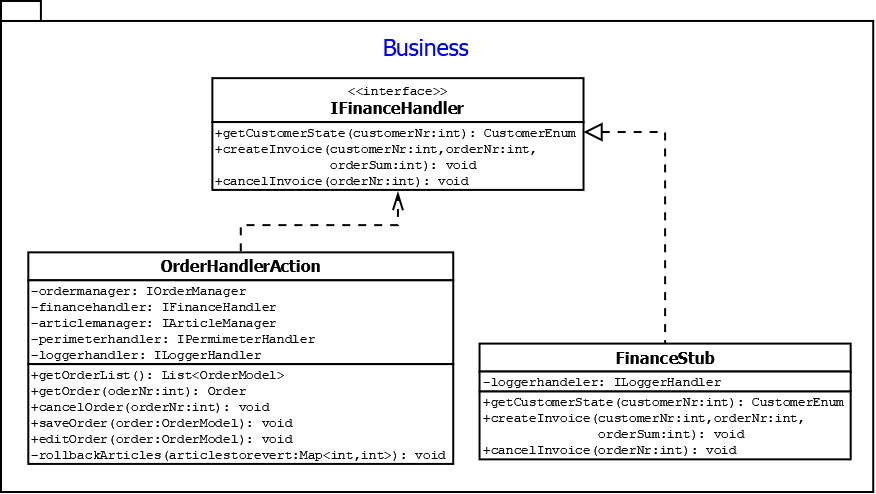
\includegraphics[width=1.0\linewidth]{Images/Zentrallager}
	\caption{Zentrallager}
	\label{fig:zentrallager}
\end{figure}



\subsubsection{Rechnungswesen}
Das Rechnungswesen hat die Aufgabe bei Erfassung / Änderung einer Bestellung eine entsprechende Rechnung an den Kunden zu versenden.\\
Von Seiten Auftraggeber sind keine Schnittstellen zur Verfügung gestellt worden und daher wurden die entsprechenden Aufgaben des Rechnungswesen als simpler Stub implementiert, der lediglich ein Output über die ausgeführte Arbeit (z.B. Neue Rechnung gedruckt) protokolliert. \\
\begin{figure}[H]
\centering
	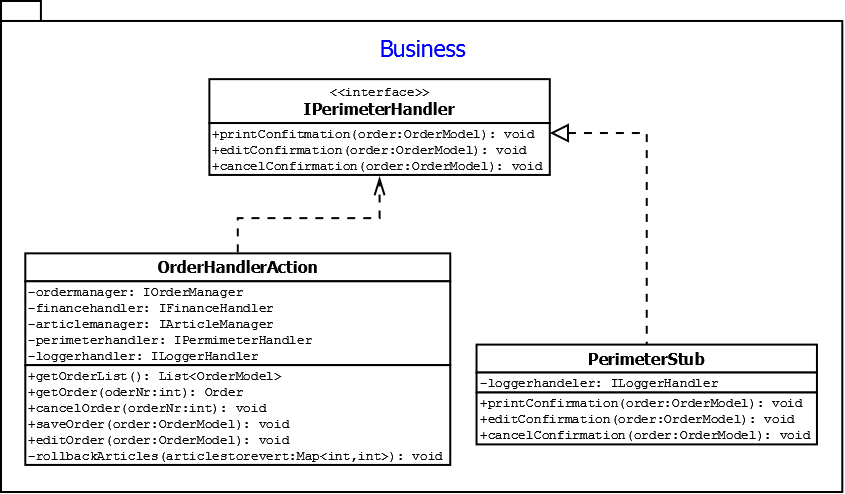
\includegraphics[width=1.0\linewidth]{Images/Rechnungswesen}
	\caption{Rechnungswesen}
	\label{fig:rechnungswesen}
\end{figure}

\subsection{Interne Schnittstellen}
In diesem Kapitel werden nur wichtige, systemrelevante Schnittstellen spezifiziert. Es werden primär die Schnittstellen zwischen den Layern 'Client', 'Business' inkl. Remote und 'Data' beschrieben.




\subsubsection{Globale Sicht}
In einer groben Übersicht wird die globale Sicht der Schnittstellen zwischen den Schichten / Packages aufgezeigt.:\\
\begin{figure}[H]
\centering
	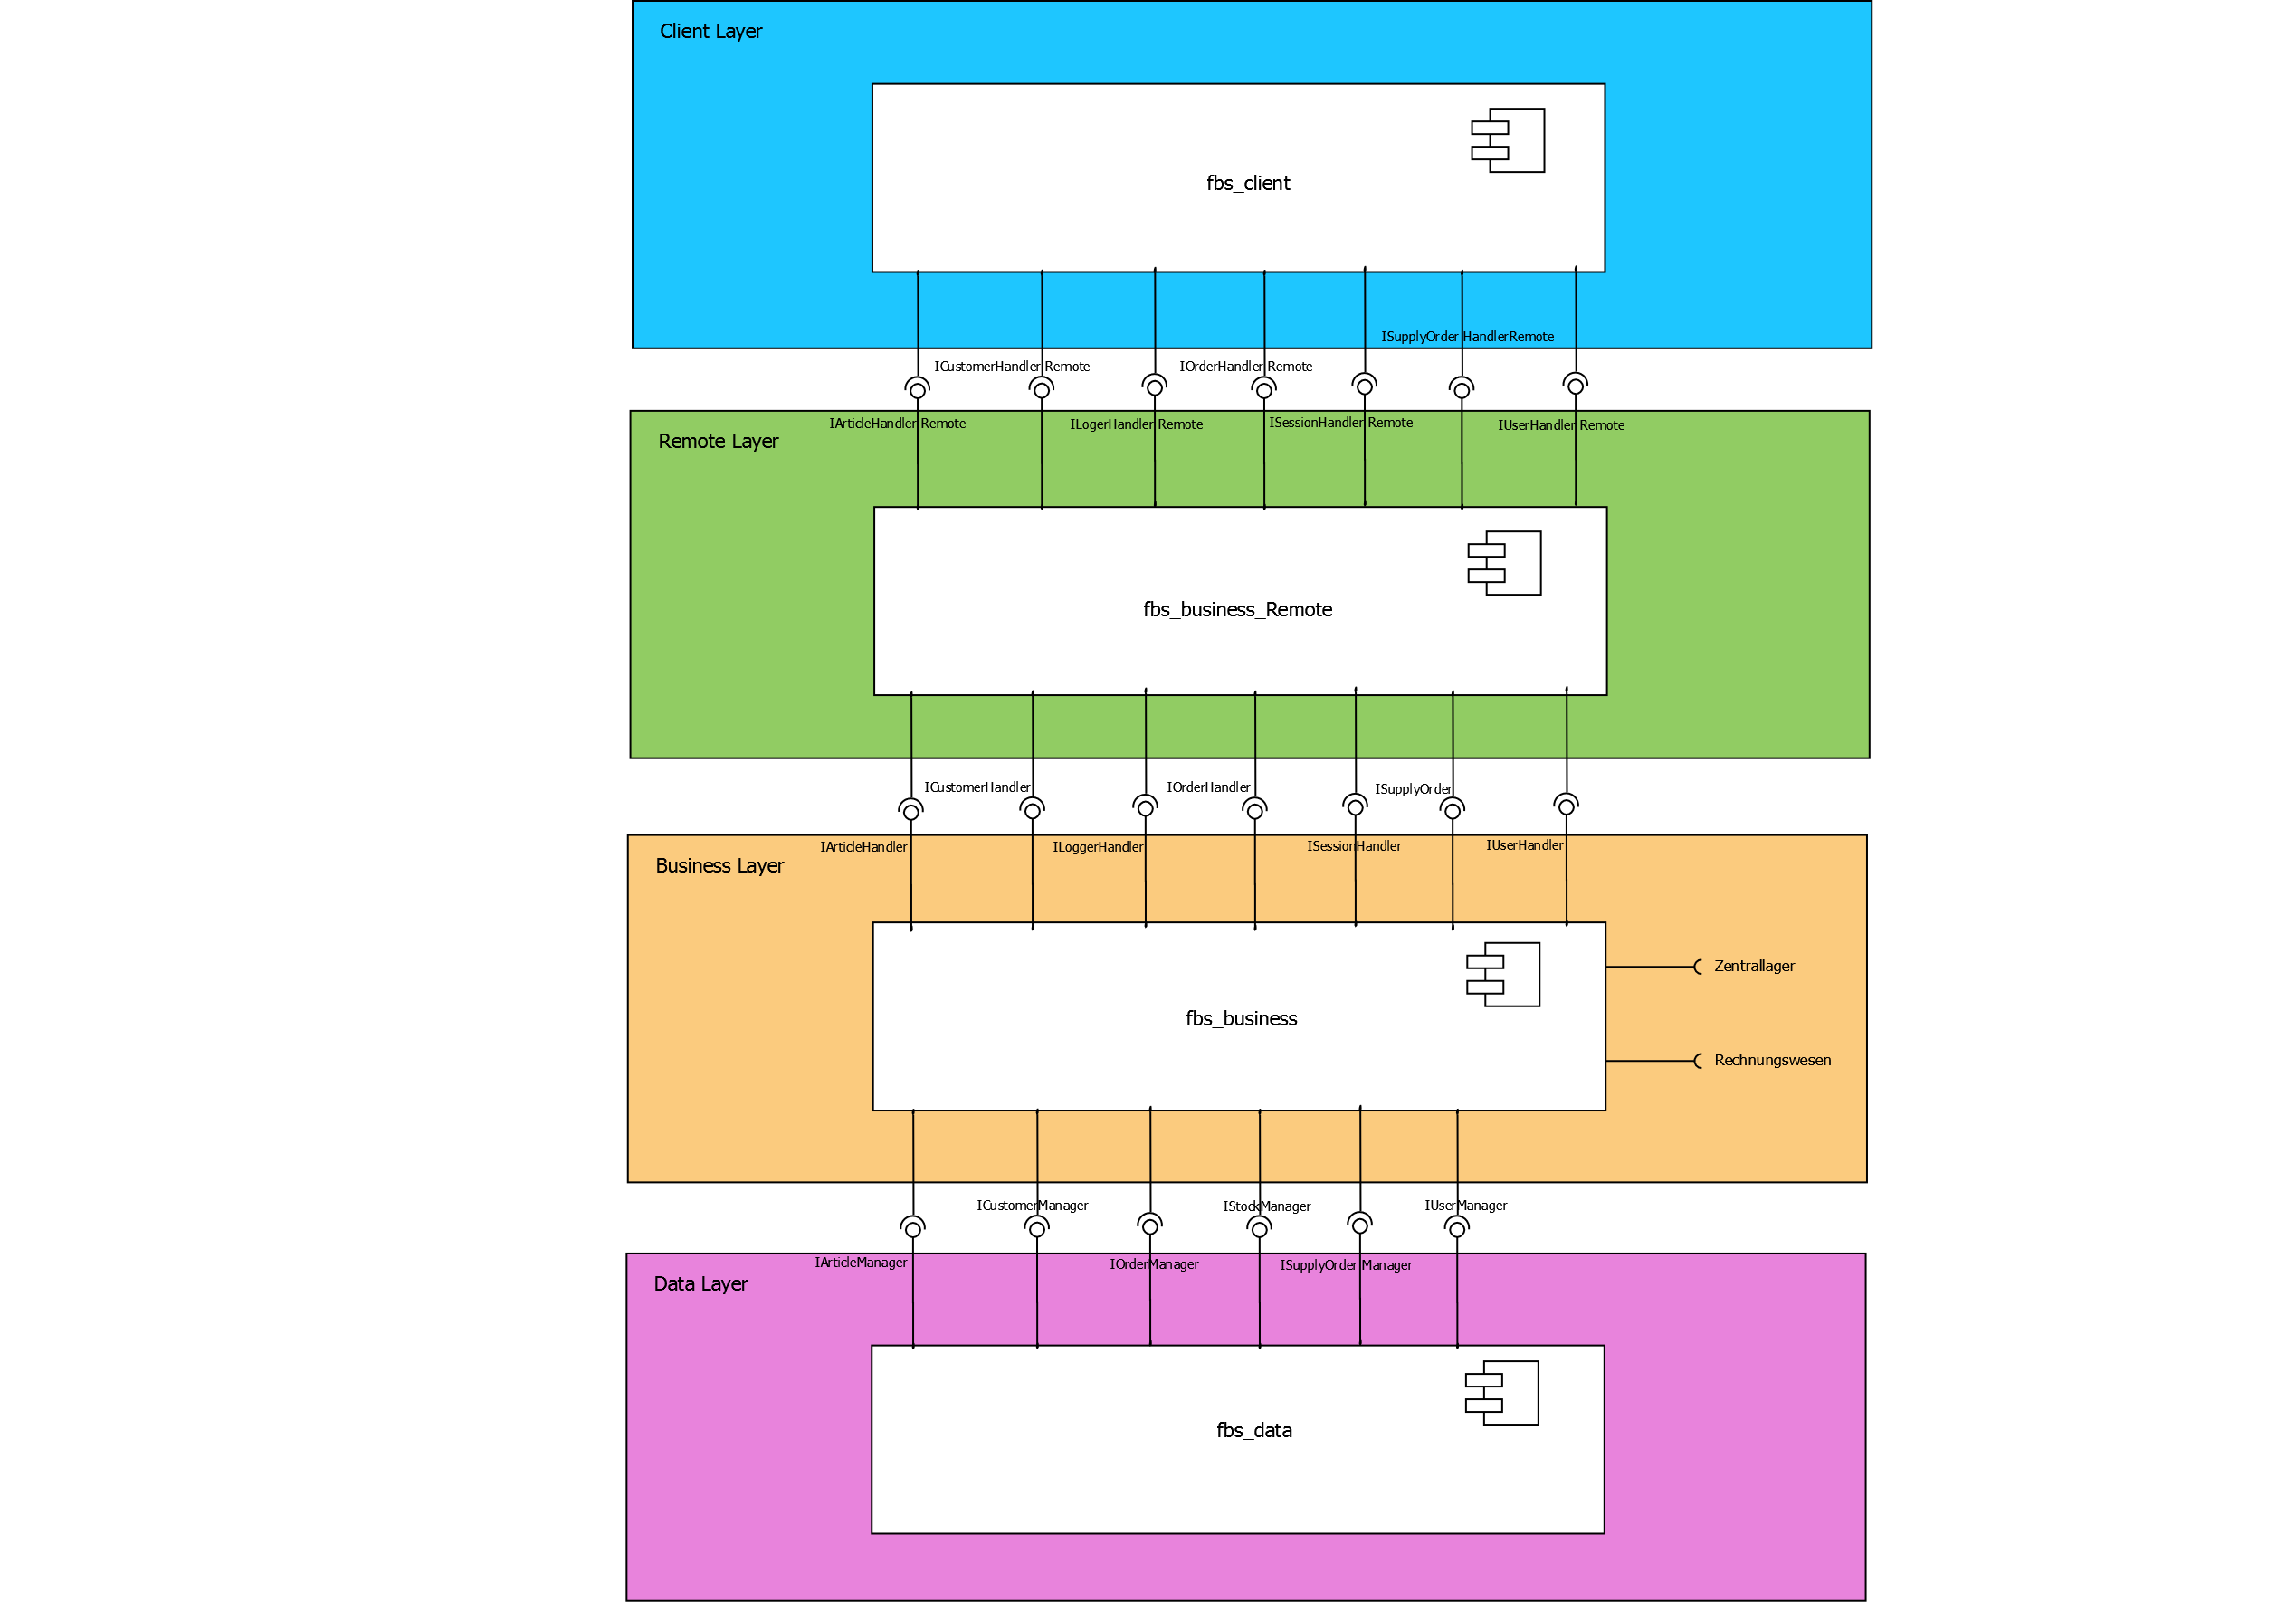
\includegraphics[width=1.0\linewidth]{Images/Schnittstellen}
	\caption{Schnittstellen}
	\label{fig:schnittstellen}
\end{figure}

\clearpage






\subsubsection{Client <-> Remote}
Zwischen der Anbindung der Layer 'Client' und 'Remote' existieren Schnittstellen, um die gewünschten Daten des Remote Layer zur Verfügung zu stellen.\\\\

\textbf{IOrderHandlerRemote}\\
Über die Methode 'getOrder' unter Angabe der gewünschten Bestellnr (int) wird vom Business Layer die Bestellung als 'OrderDTO' bereitgestellt. Für die Auflistung aller Bestellungen wird die Methode 'getOrderList' verwendet.\\
Unter Angabe der Bestellnummer kann eine Bestellung annulliert werden (Methode cancelOrder(int)). Für das Ändern oder Speichern einer Bestellung werden zusätzlich Informationen (z.B. Kunden, bestellte Artikel) benötigt, weshalb ein OrderDTO benötigt wird.


\begin{figure}[H]
	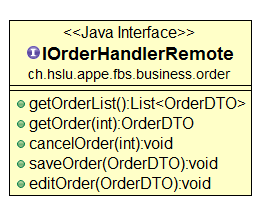
\includegraphics[width=0.3\linewidth]{Images/IOrderHandlerRemonte}
	\caption{Interface IOrderHandlerRemote}
	\label{fig:if-IOrderHandlerRemote}
\end{figure}

\textbf{ISupplyOrderHandlerRemote}\\
Für die Auflistung aller Nachbestellungen wird die Methode 'getFullOrderList' verwendet und liefert ein SupplyOrderDTO zurück.\\
Mittels der Methode 'updateSupplyFromArrical' wird mit der Übergabe eines 'SupplyOrderDTO' eine Nachbestellung ausgelöst. 
\begin{figure}[H]
	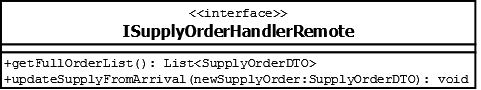
\includegraphics[width=0.6\linewidth]{Images/ISupplyOrderHandlerRemonte}
	\caption{Interface ISupplyOrderHandlerRemote}
	\label{fig:if-ISupplyOrderHandlerRemote}
\end{figure}


\textbf{IArticleHandlerRemote}\\
Für die Auflistung aller möglicher Artikel wird die Methode 'getFullArticleList' verwendet und liefert alle Liste aller verfügbaren Artikel zurück. Alle Artikel einer spezifischen Bestellung kann über 'getOrderArticleList' abgefragt werden. Sie benötigt eine ordernr (int). Ein einzelner Artikel kann über 'getArticle' mit Übergabe einer articleNr von der Remonteschicht angefordert werden. Die genannte Anzahl sind nicht garantiert, sondern zeigt lediglich einen Momentanbestand. Das Transaktionsmanagement unterliegt den unteren Layers.
\begin{figure}[H]
	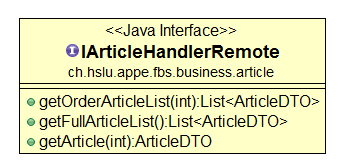
\includegraphics[width=0.6\linewidth]{Images/IArticleHandlerRemonte}
	\caption{Interface IArticlerHandlerRemote}
	\label{fig:if-IArticleHandlerRemote}
\end{figure}

\textbf{ICustomerHandlerRemote}\\
Beim ICustomerHandlerRemonte wird bis Release 1.0 keine erstellende oder mutierende Operationen angeboten. Konkret heisst dies, dass über 'getCustomerList' alle möglichen Kunden ausgewiesen werden und über eine Liste 'CustomerDTO' zurückgegeben. Es besteht mittels customerNr auch die Möglichkeit einen selektiven Kunden zu erhalten. Dies geschieht mit der Methode 'getCustomer'.
Die Methode 'getCustomerStateOK' überprüft, ob der Kunden ausstehende Mahnungen hat und liefert einen boolean (true=OK / false=Mahnung) zurück.
\begin{figure}[H]
	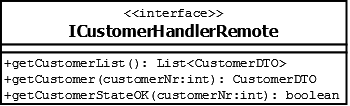
\includegraphics[width=0.4\linewidth]{Images/ICustomerHandlerRemonte}
	\caption{Interface ICustomerHandlerRemote}
	\label{fig:if-ICustomerHandlerRemote}
\end{figure}

\textbf{IUserHandlerRemote}\\
Über das IUserHandlerRemote-Interface kann Abgefragt werden ob ein User gültig ist und das richtige Passwort eingegeben wurde. Mit 'getUserRole' kann anhand des Username seine Rolle abgefragt werden, z.B. für die Auswahl der Ziel-Page. 
\begin{figure}[H]
	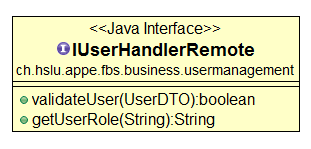
\includegraphics[width=0.4\linewidth]{Images/IUserHandlerRemonte}
	\caption{Interface IUserHandlerRemote}
	\label{fig:if-IUserHandlerRemote}
\end{figure}


\textbf{ISessionHandlerRemote}\\
Die Schnittstelle 'ISessionHandlerRemote' überprüft, ob der User die Berechtigungen für den gewünschten Ziel-Context hat oder nicht. Bei jedem Pageaufruf, wird die Überprüfung für jede Page (LoginPage ausgenommen) vorgenommen.
\begin{figure}[H]
	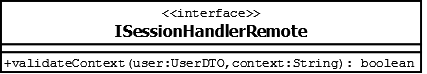
\includegraphics[width=0.5\linewidth]{Images/ISessionHandlerRemonte}
	\caption{Interface ISessionHandlerRemote}
	\label{fig:if-ISessionHandlerRemote}
\end{figure}

\textbf{ILoggerHandlerRemote}\\
Das ILoggerHandlerRemote-Interface bietet die möglichkeit anhand eines LogerDTO eine LogMessage zu übergeben. Die LogLevels werden in der unteren Schicht bestimmt. Es wird ein Default wert festgelegt für alle Log-Nachrichten vom Clint Layer.
\begin{figure}[H]
	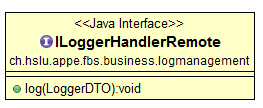
\includegraphics[width=0.5\linewidth]{Images/ILoggerHandlerRemonte}
	\caption{Interface ILoggerHandlerRemote}
	\label{fig:if-ILoggerHandlerRemote}
\end{figure}



%-----------------------------------------------------------------------




\subsubsection{Remote <-> Business}
Zwischen der Anbindung der Layer 'Remote' und 'Business' existieren ähnliche Schnittstellen wie bei 'Client <-> Remote'. Diese Schicht reicht die Client-Operationsanfragen mit notwendiger Datentransformation (DTO zu Model) an den entsprechenden Business-Handler.\\\\


\textbf{IOrderHandler}\\
Über die Methode 'getOrder' unter Angabe der gewünschten Bestellnr wird vom Data-Layer die Bestellung als 'OrderModel' bereitgestellt. Für die Auflistung aller Bestellungen wird die Methode 'getOrderList' verwendet.\\
Unter Angabe der Bestellnummer kann eine Bestellung annulliert werden (Methode cancelOrder). Für das Ändern oder Speichern einer Bestellung werden zusätzlich Informationen (z.B. Kunden, bestellte Artikel) benötigt, weshalb ein OrderModel benötigt wird. 
\begin{figure}[H]
	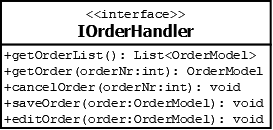
\includegraphics[width=0.3\linewidth]{Images/IOrderHandler}
	\caption{Interface IOrderHandler}
	\label{fig:if-IOrderHandler}
\end{figure}



\textbf{ISupplyOrderHandler}\\
Für die Auflistung aller Nachbestellungen wird die Methode 'getFullOrderList' verwendet.\\
Mittels der Methode 'changeLocalArticleStockAmount' wird überprüft, ob der Filiallagerbestand für jeden einzelnen Artikel unter den Mindestbestand fällt und löst bei Unterschreitung eine Bestellung beim Zentrallager aus. Die Methode 'setCurrentSupplyOrder' ermöglicht anhand der auslösenden Bestellung eine provisorische Nachbestellung zu erstellen. Alle nachzubestellende Artikel werden dieser Nachbestellung beigefügt. Nachdem alle Nachbestellartikel erfasst sind, muss diese über 'saveSupply' an den Data-Layer für die Persistierung gesendet werden. Die Methode 'updateSupplyFromArrival' wird beim Wareneingang verwendet, um angelieferte Artikel zu verbuchen. 
\begin{figure}[H]
	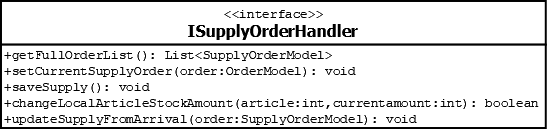
\includegraphics[width=0.6\linewidth]{Images/ISupplyOrderHandler}
	\caption{Interface ISupplyOrderHandler}
	\label{fig:if-ISupplyOrderHandler}
\end{figure}



\textbf{IArticleHandler}\\
Für die Auflistung aller möglicher Artikel (z.B. im NewOrder-Form) wird die Methode 'getFullArticleList' verwendet. Ein einzelner Artikel kann über 'getArticle' unter Artikelnummer von der Datenbank angefordert werden. Über 'getArticleAmountFromStock' kann pro Artikel der aktuelle Filiallagerbestand abgefragt werden. Die genannte Anzahl ist nicht garantiert, sondern zeigt lediglich einen Momentanbestand. Neben dem Auslesen der Artikelmenge wird über die Methode 'updateArticleAmount' die Möglichkeit zur Aktualisierung der Artikelmenge angeboten. Das Transaktionsmanagement unterliegt ausschliesslich dem Data-Layer, da über die Methode nur die gewünschte Mengendifferenz übertragen wird.
\begin{figure}[H]
	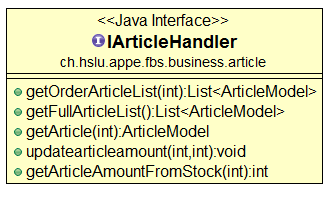
\includegraphics[width=0.6\linewidth]{Images/IArticleHandler}
	\caption{Interface IArticlerHandler}
	\label{fig:if-IArticleHandler}
\end{figure}

\textbf{ICustomerHandler}\\
Beim ICustomerHandler wird bis Release 1.0 keine erstellende oder mutierende Operationen angeboten. Konkret heisst dies, dass über 'getCustomerList' alle möglichen Kunden ausgewiesen werden. Es besteht mittels Kundennummer auch die Möglichkeit einen selektiven Kunden zu erhalten (Methode 'getCustomer).\\
Die Methode 'getCustomerStateOK' überprüft beim FinanceStub, ob der Kunden ausstehende Mahnungen hat und so nicht legitimiert ist Bestellungen zu tätigen.
\begin{figure}[H]
	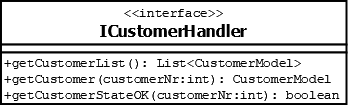
\includegraphics[width=0.4\linewidth]{Images/ICustomerHandler}
	\caption{Interface ICustomerHandler}
	\label{fig:if-ICustomerHandler}
\end{figure}
\textbf{IUserHandler}\\
Über das IUserHandler-Interface können die Userinformationen (Benutzername, Passwort und Userrolle) erfragt werden. Die Userrolle kann ebenfalls für einen bestimmten Benutzer separat erfragt werden, z.B. für die Auswahl der Ziel-Page im Client.
\begin{figure}[H]
	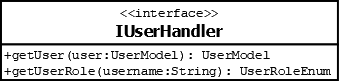
\includegraphics[width=0.4\linewidth]{Images/IUserHandler}
	\caption{Interface IUserHandler}
	\label{fig:if-IUserHandler}
\end{figure}
\clearpage
\textbf{ISessionHandler}\\
Die Schnittstelle 'ISessionHandler' überprüft, ob der User die Berechtigungen für den gewünschten Ziel-Context hat oder nicht. Bei jedem Pageaufruf, wird die Überprüfung für jede Page (LoginPage ausgenommen) vorgenommen.
\begin{figure}[H]
	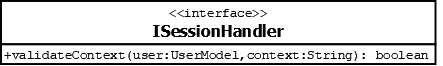
\includegraphics[width=0.5\linewidth]{Images/ISessionHandler}
	\caption{Interface ISessionHandler}
	\label{fig:if-ISessionHandler}
\end{figure}
\textbf{ILoggerHandler}\\
Das ILoggerHandler-Interface bietet anhand eines LoggerModels, welches bereits die Nachricht und Level enthält, zu übermitteln oder kann mittels dem Enum LogLevelEnum den Level und die Message als String vorgeben.
\begin{figure}[H]
	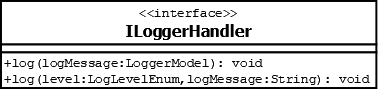
\includegraphics[width=0.5\linewidth]{Images/ILoggerHandler}
	\caption{Interface ILoggerHandler}
	\label{fig:if-ILoggerHandler}
\end{figure}

%-----------------------------------------------------------------

\subsubsection{Business <-> Data}

Zwischen der Anbindung der Layer 'Business' und 'Data' existieren Schnittstellen, um die gewünschten Daten dem Business Layer zur Verfügung zu stellen. Hier ist auch die Anbindung an die Datenbank angeordnet\\\\

\textbf{IOrderManager}\\
Über die Methode 'getOrder' unter Angabe der gewünschten OrderNr wird von der Datenenbank die Bestellung als 'OrderModel' bereitgestellt. Für die Auflistung aller Bestellungen wird die Methode 'getOrderList' verwendet.\\
Mit der Methode 'saveOrder' können neuen Order gespeichert gelöst oder aktualisiert werden. Es wird ein 'OrderModel' übergeben um die einzelnen Aktionen auszuführen. 
\begin{figure}[H]
	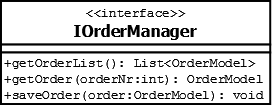
\includegraphics[width=0.3\linewidth]{Images/IOrderManager}
	\caption{Interface IOrderManager}
	\label{fig:if-IOrderManager}
\end{figure}


\textbf{ISupplyOrderManager}\\
Für eine Liste aller Nachbestellungen wird die Methode 'getFullOrderList' verwendet.\\
Mittels der Methode 'makeOrderEntry' wird eine Nachbestellung abgeschickt für die Tabelle supply. Es muss ein Artikelnummer und die Menge mitgegeben werden. Wenn einen neuen Nachbestellung gemacht werden möchte, benutzt die Methode 'saveSupplyOrder', diese verlangt ein SupplyOrderModel.
\begin{figure}[H]
	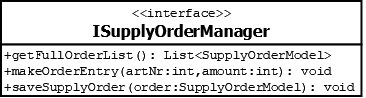
\includegraphics[width=0.6\linewidth]{Images/ISupplyOrderManager}
	\caption{Interface ISupplyOrderManager}
	\label{fig:if-ISupplyOrderManager}
\end{figure}



\textbf{ICustomerManager}\\
Beim ICustomerHandler wird bis Release 1.0 keine erstellende oder mutierende Operationen angeboten. Konkret heisst dies, dass über 'getCustomerList' alle möglichen Kunden ausgewiesen werden. Es besteht mittels Kundennummer auch die Möglichkeit einen selektiven Kunden zu erhalten (Methode 'getCustomer).\\
Die Methode 'getCustomerStateOK' überprüft beim FinanceStub, ob der Kunden ausstehende Mahnungen hat und so nicht legitimiert ist Bestellungen zu tätigen.
\begin{figure}[H]
	
\includegraphics[width=0.4\linewidth]{Images/ICustomerManager}
	\caption{Interface ICustomerManager}
	\label{fig:if-ICustomerManager}
\end{figure}



\textbf{IUserManager}\\
Über das IUserManager-Interface kann ein UserModel von der Datenbank geholt werden. Ein UserModel beinhaltet Name, Passwort und seine Rolle. Wenn der User nicht in der DB vorhanden ist wird eine Exception UserNotFoundInDatabaseExeption geworfen.
\begin{figure}[H]
	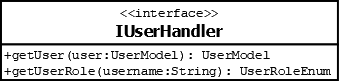
\includegraphics[width=0.4\linewidth]{Images/IUserManager}
	\caption{Interface IUserManager}
	\label{fig:if-IUserManager}
\end{figure}




\textbf{IArticleManager}\\
Das IArticleManager-Interface managt die Artikel im Data Layer und der DB. Mit der Methode 'getArticleList()' werden alle vorhandenen Artikel ('ArticleModel') zurückgegeben. Wenn auf ein spezifische Artikel benötigt wird, kann dieser mit der articleNr und der Methode 'getArticle' abgefragt werden. Mit der Methode 'getArticleAmount wird der aktuellen Lagerbestand eines Artikels zurückgegeben. Wenn neue Artikel ins lokale Lager gekommen sind, können sie mit 'updateArticleAmountInLocalStock' angepasst werden. 
\begin{figure}[H]
	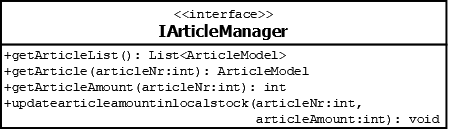
\includegraphics[width=0.6\linewidth]{Images/IArticleManager}
	\caption{Interface IArticlerManager}
	\label{fig:if-IArticleManager}
\end{figure}


\textbf{IStockManager}\\
Das Interface IStockManager besitzt die eine Methode 'getArticleAmountFromStock' und mit einer articleNr wird der Lagerbestand dieses Artikels zurückgegeben.
\begin{figure}[H]
	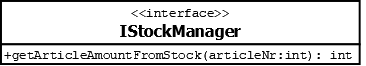
\includegraphics[width=0.5\linewidth]{Images/IStockManager}
	\caption{Interface IStockManager}
	\label{fig:if-IStockManager}
\end{figure}